The human Y chromosome carries large satellite arrays, including the centromeric DYZ3 array and the Yq12 heterochromatin, which consists mainly of DYZ1 and DYZ2 repeats (Fig.~\ref{fig:method}a and Extended Data Fig.~\ref{fig:array_structure}). DYZ3 provides the site of kinetochore assembly \cite{Jain2018}, whereas Yq12 recruits HSF1 and forms nuclear stress bodies during heat shock \cite{Penin2021}. Another array, DYZ19, lies on the long arm outside Yq12, in AZFb, a region linked to spermatogenesis \cite{Vogt2021}. Complete Y chromosome assemblies have revealed extensive variation in satellite length, with a 13.8-fold range for DYZ3 (121 kb--1.67 Mb, 123 centromeres), more than fivefold for Yq12 (10.3--53.1 Mb, 84 assemblies) \cite{Hallast2026}, and 6.7-fold for DYZ19 (63.5--428 kb, 44 assemblies, shortest in a J2a chromosome) \cite{Hallast2023}. Extending these measurements from a few hundred assembled chromosomes to the hundreds of thousands of short-read genomes linked to phenotypes in cohorts such as UK Biobank \cite{UKB2025} and All of Us \cite{AoU2024} could reveal how satellite variation relates to human traits and disease. With this goal, we developed Yruler, using pangenome assemblies to estimate the lengths of seven satellite targets, repeat composition and Y dosage in a single pass over existing short reads, without alignment.

Yruler accepts BAM, CRAM, SAM or FASTQ files and counts 31-mer markers for satellite arrays, single-copy Y regions and an autosomal window (Fig.~\ref{fig:method}b). Y markers come from pangenome assemblies \cite{Hallast2026}, using only complete satellite arrays, whereas autosomal markers come from Human Pangenome Reference Consortium (HPRC) haplotypes \cite{Lucas2026}. Y markers found in non-Y sequences of HPRC assemblies are excluded. Yruler divides G+C-corrected satellite marker counts by the single-copy Y marker count. This ratio normalizes for sequencing depth and the fraction of cells carrying Y. A separate scale factor, fitted using assembled arrays and matched short reads, converts each ratio into base pairs. Y dosage compares single-copy Y with autosomal counts, and regional Y profiles flag possible deletions and rearrangements (Extended Data Fig.~\ref{fig:chrY_unusual_males}).

We assessed accuracy for the seven satellite targets in 82--126 males per target, using ten repeats of 5-fold cross-validation with relatives kept in the same fold to prevent family overlap between training and test sets (Fig.~\ref{fig:method}b). The released model was trained on all cross-validation individuals and used for population analyses. Median absolute percentage errors ranged from 1.73\% to 3.86\%, with 90th percentiles from 4.18\% to 10.20\%. The DYZ1:DYZ2 unit ratio had a median error of 2.60\% in 82 males (Fig.~\ref{fig:method}c and Table~\ref{tab:accuracy}). Excluding each of 18 Y lineages in turn from training and predicting lengths in males of that lineage gave similar median errors overall (Extended Data Fig.~\ref{fig:lineage_validation}a).

Processing $\sim$30$\times$ whole-genome CRAMs took a median of 1.76 minutes per sample with 8 threads and 3.77 GB of peak memory (Fig.~\ref{fig:method}d). At 1$\times$ autosomal coverage, median errors ranged from 1.93\% to 4.33\% across the seven targets (Fig.~\ref{fig:method}e), and Y dosage differed from its full-depth value by a median of 0.72\% (Extended Data Fig.~\ref{fig:y_dosage}a). In 309 parent--offspring pairs from the 1000 Genomes Project \cite{ByrskaBishop2022}, median absolute percentage differences ranged from 1.8\% to 3.7\% and were 4.2\% for the DYZ1:DYZ2 unit ratio. For satellite lengths, median signed differences ranged from $-$1.1\% to 1.3\% (Fig.~\ref{fig:method}f and Extended Data Fig.~\ref{fig:pedigrees}). Five pairs differed by more than 25\% in Yq12, with an unusual Y profile in one individual and a gain of pseudoautosomal region 2 (PAR2) in two others (Extended Data Fig.~\ref{fig:chrY_unusual_males}).

A separately trained model also supports R10.4.1 nanopore reads, with median cross-validation errors 2.0--3.8 times as large as those obtained with short reads (Table~\ref{tab:ont}). In 82 males from the nanopore training panel, DYZ3 estimates agreed between platforms (Spearman $\rho$ 0.972, median absolute relative difference 6.8\%).

Previous short-read studies measured one satellite array at a time \cite{Miga2014,Altemose2014}, counted simple satellites in individual reads \cite{Said2024} or used DYZ1 read depth to approximate Yq12 length \cite{SanRoman2024}. Other k-mer methods infer centromere architecture and length for selected autosomes \cite{Hain2026}, or assign centromere haplogroups, including that of the Y chromosome, and estimate array length from a closely related reference haplotype \cite{Shiraishi2026}. We compared Yruler with the method of San Roman et al.\ on 83 males with 30$\times$ PCR-free short reads and assembled DYZ1 arrays. Their method gives relative depth, so we converted it to base pairs with a factor estimated on four fifths of the males and measured errors on the remaining fifth, using 5-fold cross-validation with relatives kept together, as for Yruler. For DYZ1, their method had a slightly lower median error than Yruler (1.76\% vs 2.25\%, P = 0.70), but its error was higher when used to estimate Yq12 length (4.17\% vs 1.73\%, 82 males, P = $1.0\times10^{-8}$).

In 1,587 males from the 1000 Genomes Project, Yruler confirmed the previously reported shorter DYZ3 arrays in R1b \cite{Hallast2023}, with a median length of 318 kb versus 979 kb in other lineages (3.1-fold) (Fig.~\ref{fig:biology}a and Extended Data Fig.~\ref{fig:population}a). The same pattern was present in the Human Genome Diversity Project (HGDP) \cite{Bergstrom2020} and the Simons Genome Diversity Project (SGDP) \cite{Mallick2016} (Fig.~\ref{fig:biology}b). We also found 3.9-fold shorter DYZ3 arrays in the East Asian lineage O2a2b1a1 than in its sister lineage O2a2b1a2 (268 vs 1,045 kb), with all sampled O2a2b1a1 arrays shorter than those in O2a2b1a2. This contrast was also seen in HGDP, SGDP and the assemblies, although sample sizes were small in SGDP (3 and 4 males) and the assemblies (3 and 2) (Fig.~\ref{fig:biology}c).

In the 1000 Genomes Project, all 42 sampled J2a1a1 chromosomes carried DYZ19 arrays 4.3-fold shorter than those of other J chromosomes (59--74 vs 222--306 kb) (Fig.~\ref{fig:biology}d and Extended Data Fig.~\ref{fig:J_DYZ19}). This extends an observation in one assembly \cite{Hallast2023} to all sampled males of this lineage, with the same pattern in HGDP and SGDP. Nanopore assemblies from the 1000 Genomes long-read resource \cite{Gustafson2024} confirmed short DYZ19 arrays in four J2a1a1 males not used for training, with lengths of 62.4--63.8 kb. A parent--offspring pair of lineage E1a2a1b2 also carried short DYZ19 arrays (83 and 77 kb; Extended Data Fig.~\ref{fig:chrY_unusual_males}). A separate analysis of aligned read depth also showed lower DYZ3 and DYZ19 read depth in the lineages with shorter arrays (Supplementary Fig.~\ref{fig:markerfree}a,b). Nanopore estimates showed the same lineage-associated patterns for DYZ3 and DYZ19, although only three O2a and six J males were available for these comparisons (Supplementary Fig.~\ref{fig:markerfree}d).

Differences between lineages accounted for 60.3\% of the variance in DYZ3 length and 76.5\% in DYZ19 length, but only 24.1--27.9\% for Yq12 and its components, which varied mostly within lineages. Yq12 contained nearly equal numbers of DYZ1 and DYZ2 units (median  DYZ1:DYZ2 unit ratio 0.97), as in assemblies \cite{Hallast2026}. The ratio differed among lineages (Kruskal--Wallis H 238.0, P $1.9\times10^{-43}$), with medians ranging from 0.88 in D to 1.05 in E (Fig.~\ref{fig:biology}e). Within lineages, DYZ2 varied more in length than DYZ1 in assemblies and all three cohorts (Fig.~\ref{fig:biology}f). Longer Yq12 arrays also had a lower DYZ1 fraction within lineages (Spearman $\rho$ $-$0.14 to $-$0.46 in the five largest lineages, Extended Data Fig.~\ref{fig:yq12_composition}b). This decrease was stronger than when DYZ2 lengths were randomly reassigned within lineages, which preserves their variation but breaks their association with the other Yq12 components (Methods).

The short-read model was trained on PCR-free Illumina libraries of cell-line DNA and is limited by the diversity of available assemblies. Arrays unlike any reference, as in 132 of 1,587 males outside the reference range, may be estimated less accurately. The model can be updated as new assemblies and sequencing data become available. Using existing sequencing reads, Yruler can bring Y satellite variation into population-scale studies of traits, disease and mosaic loss of Y.

\clearpage
\begin{figure}[tbp]
\centering
\makebox[\textwidth][c]{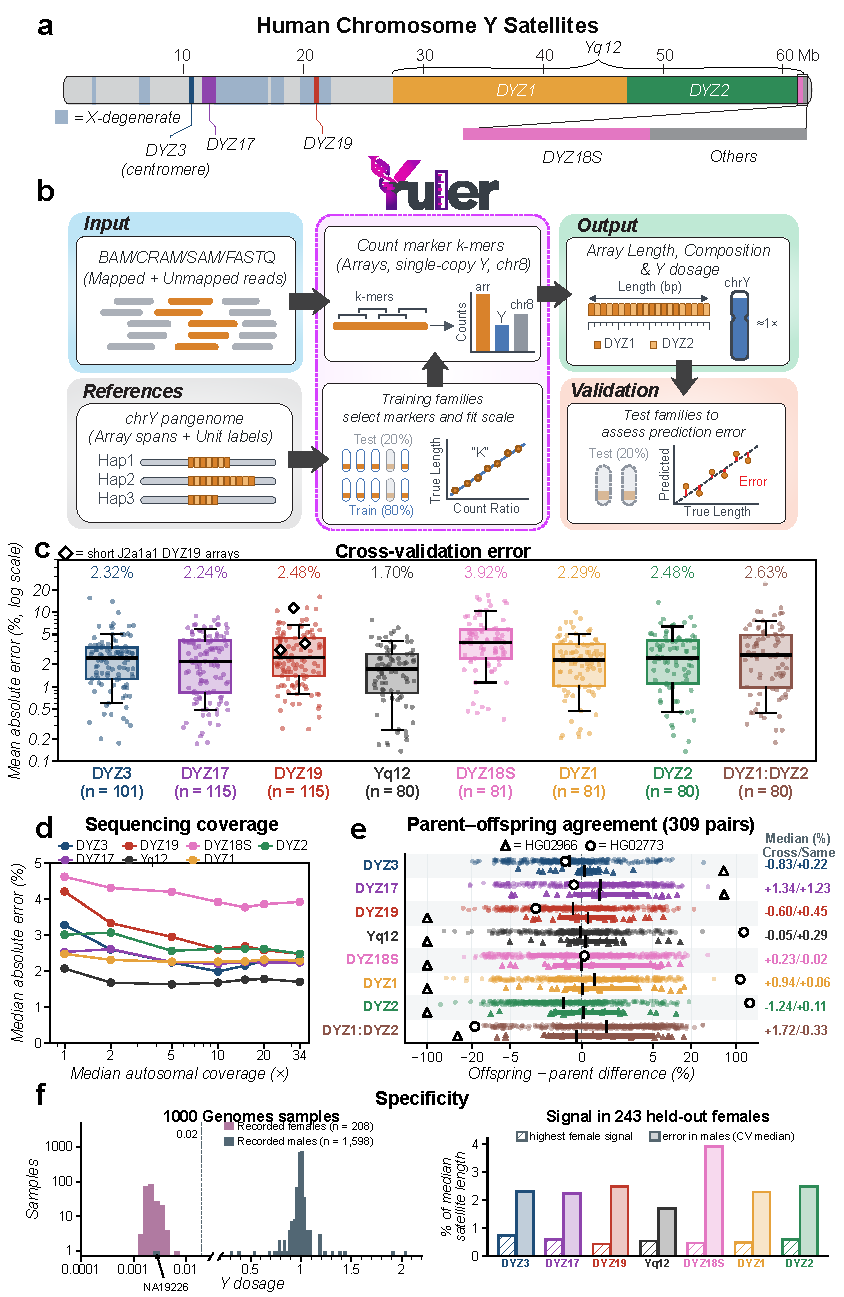
\includegraphics{figures/main/fig1_method.pdf}}
\caption{\textbf{Yruler measurement and validation.} \textbf{a}, Y satellite arrays and Yq12 components, with X-degenerate regions in blue. \textbf{b}, Workflow with family-grouped training and testing. The autosomal window is on chromosome 8. \textbf{c}, Absolute percentage errors for seven targets and the DYZ1:DYZ2 ratio. Points show each male's mean error across ten repeats of 5-fold cross-validation, and labels give pooled median errors. Diamonds: short J2a1a1 DYZ19 arrays. Logarithmic axis. \textbf{d}, Runtime and peak memory on 130 whole-genome CRAMs. In c--d, boxes show interquartile ranges, central lines medians and whiskers 10th--90th percentiles. \textbf{e}, Median errors after downsampling the test reads of the 130 cross-validation males (82 to 126 per target). \textbf{f}, Relative offspring--parent differences, $100(\mathrm{offspring}/\mathrm{parent}-1)$, in 309 pairs, with medians by batch contrast. Open triangles: HG02966. Open circles: HG02773. Scale linear within $\pm5\%$, logarithmic outside. Y dosage by sex and in read mixtures are in Extended Data Fig.~\ref{fig:no_y_cut}a,b.}\label{fig:method}
\end{figure}

\begin{figure}[tbp]
\centering
\makebox[\textwidth][c]{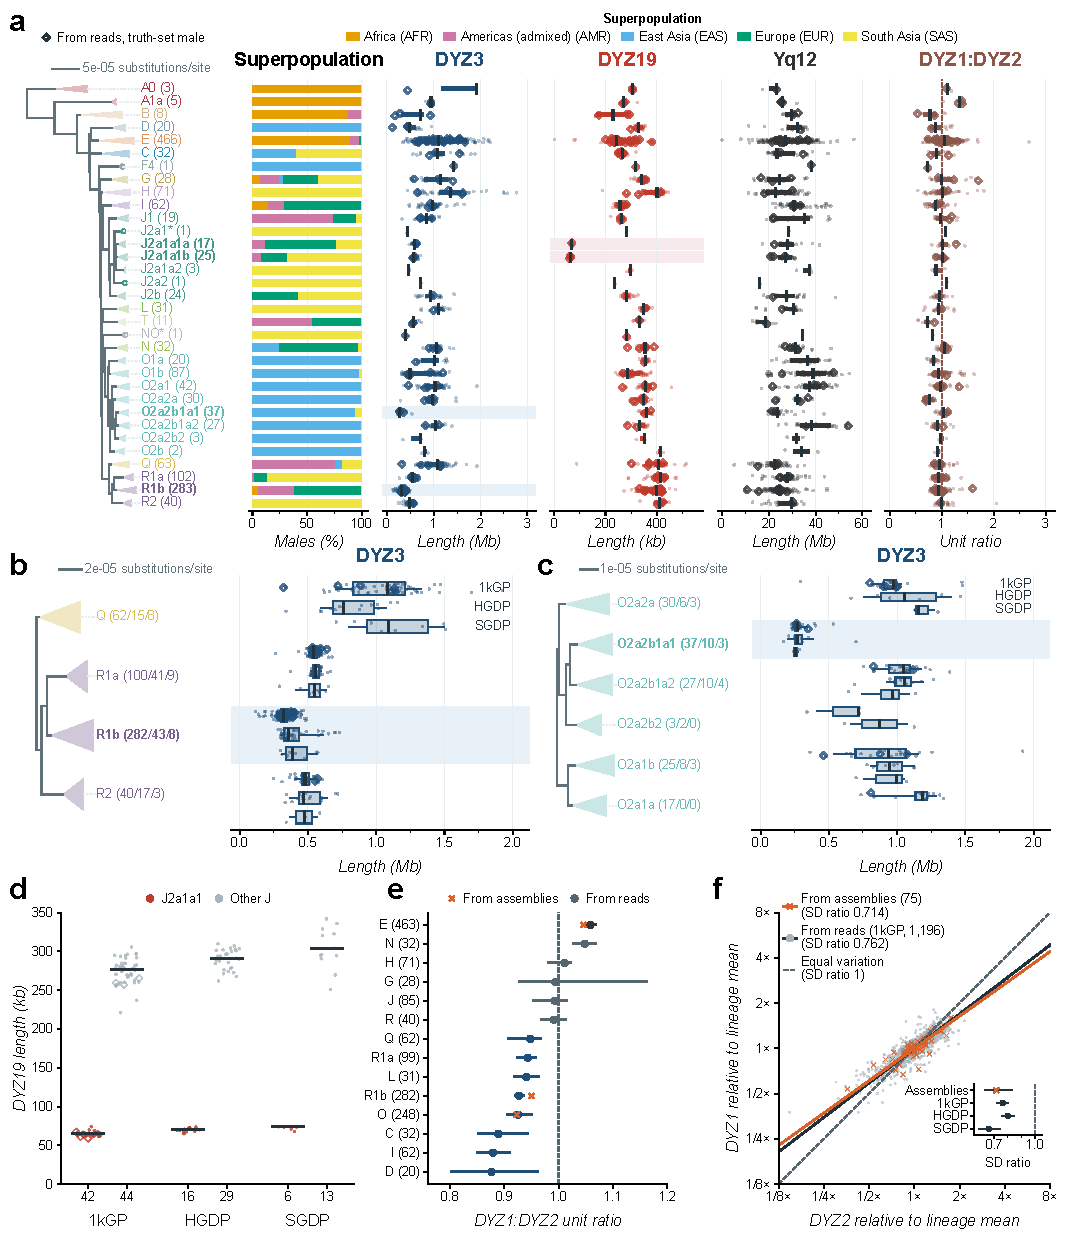
\includegraphics{figures/main/fig2_biology.pdf}}
\caption{\textbf{Y satellite variation across paternal lineages.} \textbf{a}, Single-nucleotide polymorphism (SNP) tree of 1,597 1000 Genomes Project (1kGP) males, with collapsed haplogroup clades, cohort-reported superpopulation proportions and satellite measurements. Counts in brackets give the males of each clade in the tree. Bars show interquartile ranges and ticks medians for clades with at least five males, over the 1,587 males of the population summaries, or 1,583 for Yq12 and the ratio. Shading highlights R1b and O2a2b1a1 in DYZ3, and J2a1a1 in DYZ19. \textbf{b}, DYZ3 in R1b and other lineages by cohort. \textbf{c}, DYZ3 in O2a clades, with cohorts ordered 1kGP, HGDP, SGDP. Boxes show interquartile ranges, central lines medians and whiskers 10th--90th percentiles. \textbf{d}, DYZ19 in J2a1a1 and other J lineages, excluding four Yp-depleted males from 1kGP. Fold annotations give ratios of group medians, and numbers indicate sample sizes. \textbf{e}, DYZ1:DYZ2 unit ratios from reads (dots, medians and 95\% intervals from resampling kinship components) and assemblies (crosses). Dashed line: equal numbers of units. \textbf{f}, DYZ1 and DYZ2 lengths divided by their lineage geometric means, on logarithmic axes, in 1,186 1kGP males without reference assemblies and 83 assemblies \cite{Hallast2026}. Lines have slopes SD(log DYZ1)/SD(log DYZ2), with SD the standard deviation, with 1 indicating equal variability. Inset: ratios for assemblies and the three cohorts (HGDP 386 males, SGDP 151), with 95\% bootstrap intervals. Open diamonds in a--d mark individuals with reference assemblies for that target. These estimates may be in-sample. Tests in b--d are two-sided Mann--Whitney tests and in f Pitman--Morgan tests, with P values in the Methods; 1kGP tests use one male per kinship component.}\label{fig:biology}
\end{figure}
